\documentclass[11pt,a4paper]{article}
\usepackage[T1]{fontenc}
\usepackage{graphicx}
\usepackage{mathtools}
\usepackage{amssymb}
\usepackage{geometry}
\usepackage{titlesec}
\usepackage{enumitem} % 添加enumitem宏包
\usepackage{amsfonts}
\usepackage{amssymb}
\usepackage{fancyhdr} % 添加fancyhdr宏包
\usepackage{lastpage} % 添加lastpage宏包
\usepackage{graphicx} % 导入graphicx包
\usepackage{gensymb} % 引入gensymb包
\usepackage[UTF8]{ctex}
% 应用fancyhdr宏包的页脚样式
\pagestyle{fancy}
\fancyhf{} % 清除当前的页眉页脚设置
\fancyfoot[L]{免费开源,请勿商用} % 页脚左下方显示文字
\fancyfoot[R]{作者:阿尧} % 页脚右下方显示文字
\renewcommand{\headrulewidth}{0pt} % 去掉页眉的横线
\renewcommand{\footrulewidth}{1pt} % 设置页脚的横线宽度
\usepackage{draftwatermark} %增加水印
\SetWatermarkText{本真题由b站up陈瀚尧探索世界免费开源}
\SetWatermarkScale{0.3} % 可以调整为合适的大小
\SetWatermarkColor{gray!50} % 灰色透明度为50%

% 设置更窄的页面边距
\geometry{left=3cm, right=3cm, top=1cm, bottom=2cm}

% 设置section标题格式
\titleformat{\title}{\bfseries}{\thetitle}{1em}{}

% 设置section之间的距离
\titlespacing*{\section}{0pt}{3.25ex plus 1ex minus .2ex}{1.5ex plus .2ex}

\begin{document}
    \title{中国科学院大学\\2016年招收攻读硕士学位研究生入学统一考试试题\\科目名称:光学}
    \author{制作者:b站up 陈瀚尧探索世界}
    \date{}
    \maketitle
    % 设置section标题不显示序号
    \titleformat{\section}[block]{\normalfont\Large\bfseries}{}{0pt}{}

    % 设置itemize环境的项目符号为空
    \setlist[itemize]{label=} 

    \section{考试须知:}
    \begin{itemize}[topsep=0pt,itemsep=0pt,partopsep=0pt]
        \item 1.本试卷满分为150分,全部考试时间总计180分钟。
        \vspace{-3mm}
        \item 2.所有答案必须写在答题纸上,写在试题纸上或草稿纸上一律无效。
        \vspace{-3mm}
        \item 3.可以使用无字典存储或编程功能的电子计算器。(此条对于25考研可能作废)
    \end{itemize}
    \vspace{-5mm}
    \noindent\rule{\textwidth}{0.5pt} % 添加一条线
    \vspace{-12mm}
    \section*{1、填空(共12分,每小题2分)}
    \begin{itemize}
        \vspace{0mm}
        \item (1)发生全反射的条件是\underline{\makebox[2cm]{}}和\underline{\makebox[2cm]{}}
        \vspace{0mm}
        \item (2)假定某人在白天的瞳孔直径为2mm,在夜晚的瞳孔直径为5mm,则此人在白天的极限分辨角是\underline{\makebox[2cm]{}},在夜晚的极限分辨角是\underline{\makebox[2cm]{}}。
        \vspace{0mm}
        \item (3)照相物镜的相对孔径是\underline{\makebox[2cm]{}},显微物镜的数值孔径是\underline{\makebox[2cm]{}}
        \vspace{0mm}
        \item (4)对于正常人眼,要观察1m远的目标,需要调节\underline{\makebox[2cm]{}}视度。一个人的远点距离为$-0.5m$,需配的眼镜为\underline{\makebox[2cm]{}}“度”近视镜。
        \vspace{0mm}
        \item (5)在一个$3^{x}$的伽利略望远镜物镜前,加一个焦距为150mm的正透镜,则此组合放大镜的视放大率是\underline{\makebox[2cm]{}}倍。
        \vspace{0mm}
        \item (6)光学系统的单色像差有\underline{\makebox[2cm]{}},\underline{\makebox[2cm]{}},\underline{\makebox[2cm]{}},\underline{\makebox[2cm]{}},\underline{\makebox[2cm]{}}五种;色差有\underline{\makebox[2cm]{}},\underline{\makebox[2cm]{}}两种。
        \vspace{0mm}
    \end{itemize}
    \section*{二、画图题(同2019年)}
    \begin{itemize}
        \item (1) 用作图法求图中垂轴像A'B'对应的物AB
        
        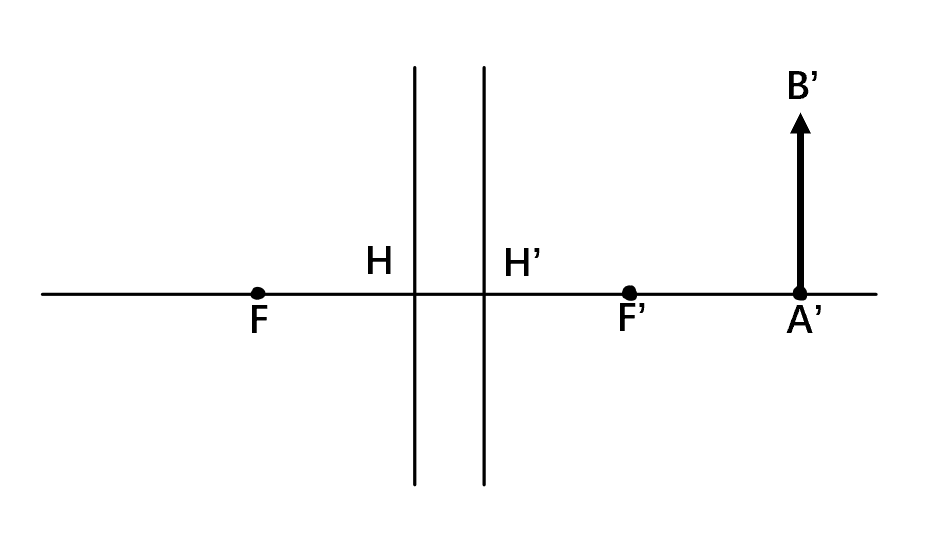
\includegraphics[scale=0.2]{1.png}% 插入图片,按50%的比例缩放
        \vspace{-5mm}
        \item (2) 用作图法求下图薄透镜的焦点F, F'的位置。
         
        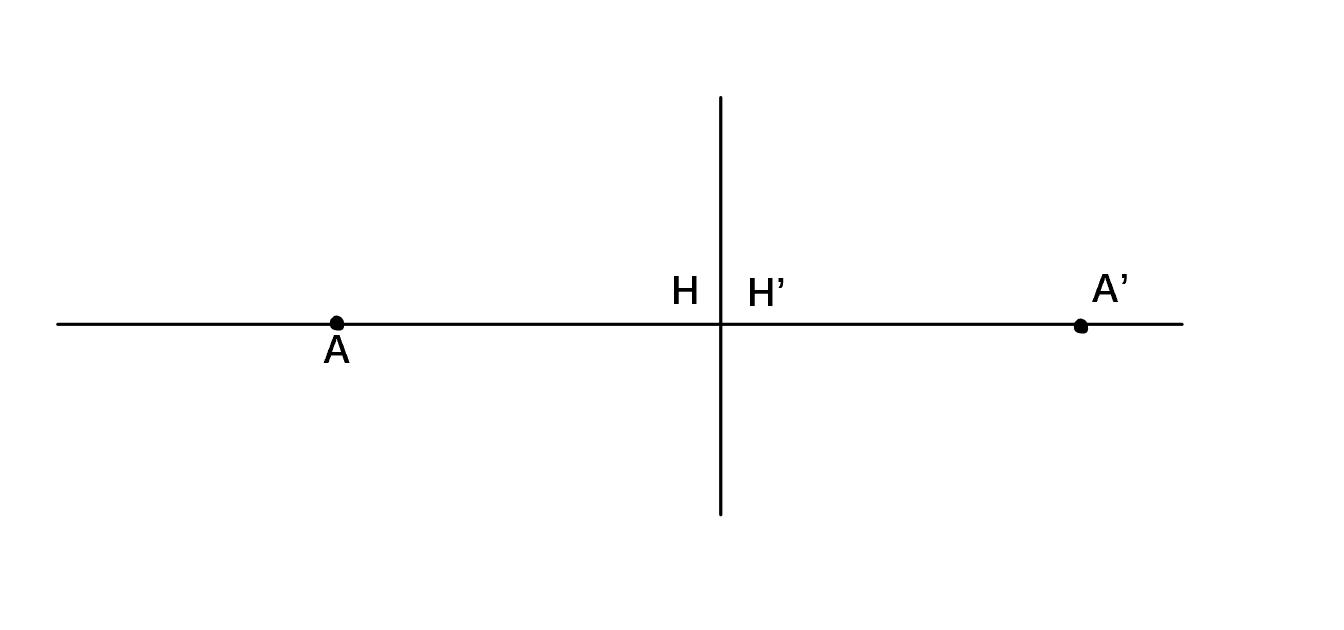
\includegraphics[scale=0.2]{2.png}% 插入图片,按50%的比例缩放
        \vspace{-5mm}
        \item (3) 用作图法求图中垂轴物体AB的像A'B'
        
        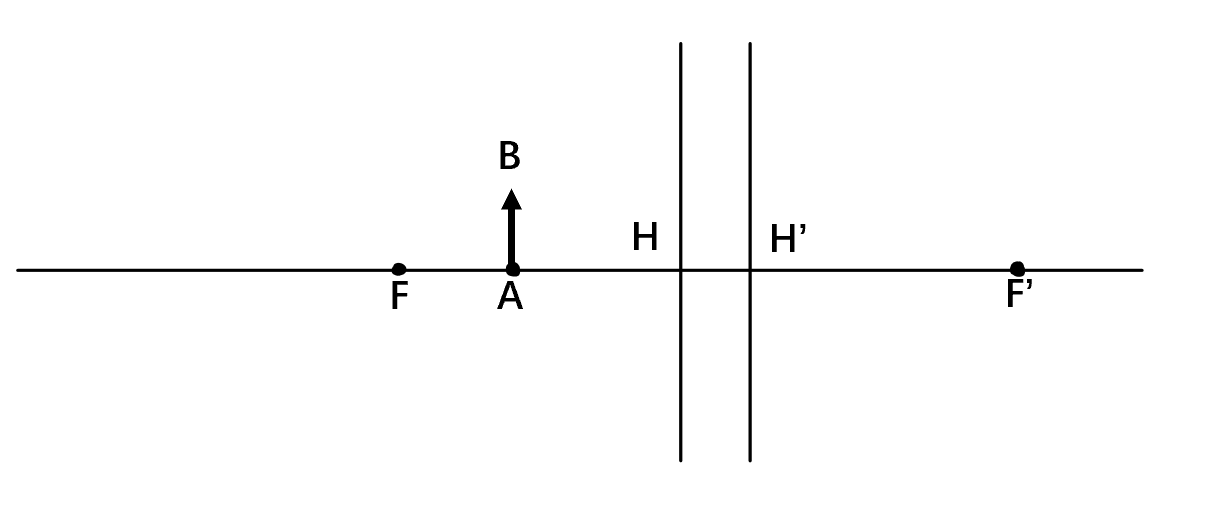
\includegraphics[scale=0.2]{3.png}% 插入图片,按50%的比例缩放
    \end{itemize}
    \vspace{10mm}
    \subsection*{3.一个正透镜焦距为100mm,一根小木棒40mm,平放在透镜的光轴上,木棒中点距离透镜200mm,求:}
    \begin{itemize}
        \vspace{0mm}
        \item (1)木棒像的长短;
        \vspace{0mm}
        \item (2)木棒绕中心转$90\degree $时,木棒像的位置和大小。
    \end{itemize}
    \vspace{20mm}
    \subsection*{4.凹面反射镜的半径为$-400mm$,物体放在何处可以成放大两倍的实像?放在何处可以成放大两倍的虚像?}
    \vspace{20mm}
    \subsection*{5.有一物镜焦距$f^{'}=100mm$,其框直径$D=40mm$,在它前面50mm处有一光阑孔,直径$D_1=35mm$}
    \begin{itemize}
        \vspace{0mm}
        \item (1)对于轴上物点,位于透镜前500mm时,系统的入瞳和出瞳位置及大小;
        \vspace{0mm}
        \item (2)对于轴上物点,位于透镜前300mm时,系统的入瞳和出瞳位置及大小;
    \end{itemize}
    \vspace{20mm}
    \subsection*{6.波长为$0.5\mu m$的平行光线由空气以$30\degree$角通过厚度为1mm、折射率为1.5的平行平板,其相位改变多少?}
    \vspace{20mm}
    \subsection*{7.一电矢量与入射面成$30\degree$角的线偏振光,以$60\degree$角斜入射到玻璃-空气界面上,玻璃和空气的折射率分别为1.5和1。试确定反射光的偏振状态。}
    \vspace{20mm}
    \subsection*{8.今在平板玻璃片上镀一层银膜,然后在银膜上加镀一层透明介质膜,在其上再镀一层银膜,制成一块干涉滤光片。设银膜的反射率为0.95;透明介质膜的折射率为1.56,膜厚为$0.4\mu m$。若用一束平行光垂直照射该干涉滤光片,求在$380.0~760.0nm$可见光范围内,透射最强的光谱线数目,相应的波长和谱线的线宽。}
    \vspace{20mm}
    \subsection*{9.杨氏实验中,点光源发出中心波长为$\lambda_0=500nm$的照明光波波列,并在观察屏上最多看到了50条亮纹,试确定该光源产生的波列谱线宽。}
    \vspace{20mm}
    \subsection*{10.正常条件下,人眼瞳孔直径约为2.5mm,人眼最灵敏的波长为550nm。}
    \begin{itemize}
        \vspace{0mm}
        \item (1)试求人眼的最小分辨角;
        \vspace{0mm}
        \item (2)若要分辨开远处相距0.5m的两个光点,人眼应距离光点多远?
        \vspace{0mm}
        \item (3)若要借助望远镜分辨开角距离为$3*10^{-7}rad$的两颗星,其物镜的最小直径是多少?为充分利用望远镜的分辨本领,该望远镜的放大率应为多大?
    \end{itemize}
    \vspace{20mm}
    \subsection*{11.一光栅宽为5cm,每毫米内有500条刻线。当用波长为500nm的平行光垂直照射时,其第三级衍射光谱缺级。试求:}
    \begin{itemize}
        \vspace{0mm}
        \item (1)光栅每个缝的宽度;
        \vspace{0mm}
        \item (2)光栅第二级衍射光谱的半角宽度;
        \vspace{0mm}
        \item (3)光栅第二级可分辨的最小波长差。
    \end{itemize}
    \vspace{20mm}
    \subsection*{12.一细光束掠入射厚度为5cm的单轴晶体平行平板,晶体的光轴与入射面垂直。若$n_o=1.525$,$n_e=1.479$,试计算在第二个面上输出两个光分开的距离,并绘出光路图。}
    \vspace{20mm}
    \subsection*{13.今利用起偏器和石英薄片产生一束右旋(按逆光传播方向定义)椭圆偏振光,其椭圆的长轴在光轴方向上,长短轴之比为2:1。试绘图说明起偏器和石英薄片如何放置,并计算石英薄片的厚度。(设光波长$\lambda=0.5893\mu m$,石英的主折射率$n_o=1.5442$,$n_e=1.5533$。)(14分)}
    \vspace{20mm}
\end{document}